\chapter{Approach}\label{approach}

\section{Quadrotor Platform}
Because the design and construction of a quadrotor is beyond the scope of  this research project, we will use a commercially available vehicle called the Bitcraze Crazyflie \cite{bitcraze}. The Crazyflie, shown in Figure \ref{fig:quad} is a small, low cost, open-source quadrotor kit suitable for indoor flight. It measures 9 cm motor to motor and weighs 19 grams. A 170 mAh lithium-polymer battery powers the vehicle, providing 7 minutes of flight time. An onboard microcontroller is responsible for vehicle stabilization and control and reads sensor measurements from a three-axis accelerometer and a three-axis gyroscope.
\begin{figure}[!htb]
\centering \includegraphics[scale=.11]{../fig/crazyflie.jpg}
\caption{Bitcraze Crazyflie Quadrotor}
\label{fig:quad}
\end{figure}

Vehicle pitch, roll, yaw, and thrust inputs are set in one of two ways. First, a USB gamepad connected to a computer running the Crazyflie PC client provides a method for direct user control of the vehicle. Second, the PC client exposes a Python API, making it possible to programmatically send the vehicle control set-points. The vehicle receives control inputs and transmits telemetry data wirelessly over a 2.4 GHz radio connection to a USB radio dongle connected to the Crazyflie PC client running on a laptop computer.

The onboard stabilization and control system implements an outer-loop attitude controller and an inner-loop rate controller, as shown in Figure \ref{fig:control_system_block_diagram}. Reference pitch and roll commands ($\theta$ and $\phi$, respectively) are fed to the attitude controller, which outputs desired rates to the rate controller. The reference yaw rate ($\dot\psi$) is fed directly to the rate controller. The outer-loop attitude control operates at 250 Hz and the inner-loop rate control operates at 500 Hz.
\begin{figure}[htb!]
	\centering
	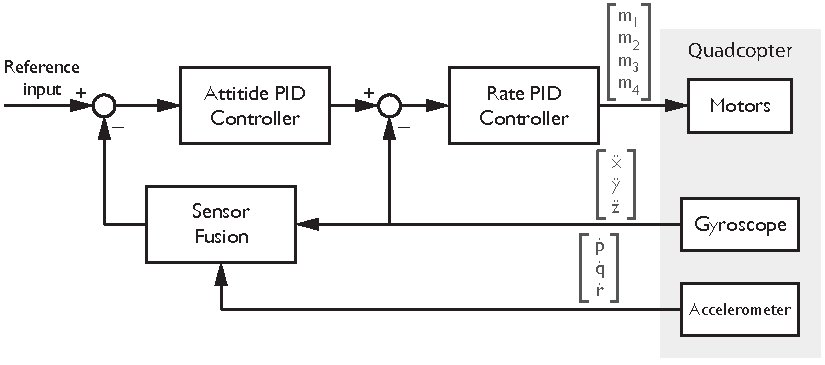
\includegraphics{../fig/crazyflie_control_system_block_diagram.pdf}
	\caption[Crazyflie stabilization and control system block diagram.]{Crazyflie stabilization and control system block diagram where $m = \begin{bmatrix}u_1 & u_2 & u_3 & u_4\end{bmatrix}^T$ is a vector of motor commands, $\ddot r = \begin{bmatrix}\ddot{x}&\ddot{y}&\ddot{z}\end{bmatrix}^T$ is a vector of vehicle accelerations, and $\dot\Theta = \begin{bmatrix}p & q & r\end{bmatrix}^T$ is a vector of vehicle angular velocities.}
	\label{fig:control_system_block_diagram}
\end{figure}


\section{Experimental Collection of Closed-Loop Input-Output Data}
All system identification methods rely on a rich set on input-output data. In order to develop a robust system model, the input sequence must sufficiently excite all system modes to be identified and the sensor data must be sampled fast enough to avoid aliasing. Because the choices made during the process of experimental data collection have a direct impact on the identified model, it may be necessary to update aspects of the collection approach if the model is found to be insufficient. In this sense, the development of a system model through system identification may be viewed as an iterative process.

\subsection{Input Design}
The input sequence used to excite the system to be modeled plays an important role in solving the identification problem. Common input sequences used for system identification include impulse signals, doublets, white-noise sequences, frequency sweeps, and Pseudo-Random Binary Sequences (PRBS) \cite{verhaegen2007filtering}. We defined three major requirements for selecting an input sequence:
\begin{enumerate}
\item The sequence must be capable of sufficiently exciting all system modes to be identified.
\item The sequence must meet the persistence of excitation criteria established by Assumption 4 in Section \ref{sec:closed-loop_subspace_identification}.
\item The sequence must be either simple enough to manually execute via direct user control or formatted in such a way that it is easily transmitted to the vehicle for execution.  
\end{enumerate}
Considering the above factors, we chose to use a PRBS signal for system input. A PRBS signal, shown in Figure \ref{fig:general_prbs}, is persistently exciting to the order of the period of the signal \cite{wilson2005understanding} and is easily transmitted to the Crazyflie quadcopter by sending input sequences using the Python API\@.
\begin{figure}[htb!]
	\centering
	
\includegraphics{../fig/general_prbs.eps}
	\caption{A general Pseudo-Random Binary Sequence.}
	\label{fig:general_prbs}
\end{figure}

We generated the PRBS signals used for identification by using the \matlab System Identification Toolbox, specifying the signal period to ensure the persistence of excitation criteria is met. Signals were generated for pitch, roll, and yaw rate. Additional input conditioning was performed to appropriately scale the magnitude of the input signal. Scaling factors were experimentally determined to sufficiently excite the vehicle's dynamics without rendering it uncontrollable.

\begin{table}[!htb]
\centering
\caption{PRBS Scaling Factors}\vspace{1em}
\begin{tabular}{lcc}
\toprule
Input & Maximum & Minimum\\
\midrule
Pitch & $+25^\circ$ & $-25^\circ$\\
Roll & $+25^\circ$ & $-25^\circ$\\
Yaw Rate & $+50^\circ/\mbox{sec}$ & $-50^\circ/\mbox{sec}$\\
\bottomrule
\end{tabular}
\end{table}

\begin{figure}[htb!]
	\centering
	\includegraphics{../fig/test_prbs.eps}
	\caption[A sample PRBS signal used for identification showing scaled inputs for vehicle pitch, roll, and yaw rate.]{A sample PRBS signal used for identification showing scaled inputs for vehicle pitch $= \pm 25^\circ$, roll $= \pm 25^\circ$, and yaw rate $= \pm 50^\circ/\mbox{sec}$.}
\end{figure}

Because the Python API requires system input sequences to be formatted as \{pitch, roll, yaw rate, thrust\}, we also experimentally determined a thrust input which results in vehicle hover. The general flight test sequence is then: vehicle power on and sensor calibration, take off and hover to an elevation where the vehicle is no longer experiencing ground effect, free flight under PRBS input, landing and vehicle power off. It is worth nothing that the PRBS input does not drive the vehicle directly, instead it acts as a reference input to the controller which in turn commands the vehicle motors. By recording the controller output and using it as system input for the purposes of identification, we ensure that the vehicle is operating under feedback control and the input-output data gathered is in fact closed-loop data.

\subsection{Data Collection}
System identification requires a rich set of input-output data to identify a suitable model. The Nyquist sampling theorem requires us to sample data at a rate higher than the Nyquist frequency in order to ensure we are able to adequately reconstruct the system input and output signals from logged data \cite{franklin1998digital}. In the case where the full system dynamics are unknown, it is not trivial to exactly identify the Nyquist frequency. Instead, we sample data at a sufficiently fast rate to identify all system dynamics we are interested in modeling. 

The PC client logging framework provides a means to log system parameters including motor inputs and onboard sensor measurements. The Crazyflie PC client communicates with the vehicle and receives logged telemetry data using a custom protocol called the Crazy Real Time Protocol (CRTP). CRTP packets are able to carry a maximum of 31 bytes of data and radio bandwidth is user configurable to either 250 kbps, 1 Mbps, or 2 Mbps. The CRTP protocol is configured to give highest priority to user inputs and as a result, may drop non-essential packets including log packets if bandwidth is constrained. In order to maximize data logging ability and minimize dropped log packets, we configure the radio to operate at 2 Mbps and send the vehicle input commands at 10 Hz. Because the log packets are limited to 31 bytes, we split the logged variables into three separate packets as follows: one log packet contains motor input commands for each of the four motors, one log packet contains $x$, $y$, and $z$ acceleration measurements, and one log packet contains pitch, roll, and yaw rate measurements from the gyroscope. As a result of the packet size limitation and the need to transmit logged variables in three separate packets, the fastest we are were to reliably log data was 50 Hz.
\begin{table}[!htb]
\centering
\caption{Logging configuration.}
\begin{tabular}{p{7em}p{17em}c}
\toprule
Quantity & Value & Logging Frequency\\
\midrule
Motor inputs & Integers of the input command sent to each of the four motors. Values range from 0 to 64000. & 50 Hz \\[5em]
Accelerometer measurements & Measurements of $x$, $y$, and $z$ accelerations in terms of G's (measured value normalized for gravity) & 50 Hz\\[3em]
Gyroscope \hspace{2em}measurements & Measurements of pitch, roll, and yaw rates in degrees/second. & 50 Hz\\
\bottomrule
\end{tabular}
\end{table}

A suitable test flight location minimizes the introduction of additional disturbances during data collection. In order to avoid the introduction of disturbances from air turbulence and wind gusts, we performed all test flights indoors. Performing all flights on the same day and with a fully charged quadrotor battery further added to the consistency of the data collected. Test flight length limitations arise from physical room size constraints and battery capacity. The vehicle tends to drift under PRBS inputs, forcing the termination of a test flight any time the vehicle approaches a physical obstacle or wall. Flight tests were conducted in a large, open room to maximize test flight duration. 

\section{Data Analysis}
Prior to building a model from the sampled data, the raw data is conditioned to provide a more consistent estimate of system dynamics. Following data preprocessing, we performed model identification offline using a finite number of sampled data points.


\subsection{Data Preprocessing}
Before identifying a system model, we preprocessed the data to make it suitable for use. First we trimmed the beginning and end of the collected input-output sequences to recover only the data collected when the vehicle was driven by PRBS inputs. This process was achieved by simultaneously plotting all input-output data and visually identifying the beginning and end of the data sequences to retain.
\begin{figure}[htb!]
	\centering
	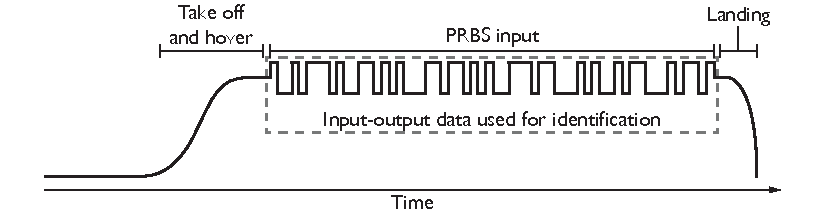
\includegraphics{../fig/test_flight_profile.pdf}
	\caption{Quadrotor test flight profile showing the portion of the test flight data used for system identification.}
	\label{fig:test_flight_profile}
\end{figure}

After extracting the usable segment of the collected data, it was time normalized. SIMs require the input-output data to be uniformly sampled with data points aligning in time. Because the Crazyflie logging framework does not guarantee data is measured and logged simultaneously, we normalized the sampling times by applying a zero-order hold and resampled the data using a common time vector at a uniform rate of 50 Hz.


\subsection{Model Identification}
We identified a model of the unknown system by applying the IEM according to the general procedure outlined in Table \ref{iem_overview}. A custom \matlab script processed the data offline and presented results when the algorithm was complete. Before identifying a model, selection of system order and past and future horizons was made. The system order was determined from a plot of the singular values of the extended observability matrix and past and future horizon values were selected as described in Section \ref{sec:past_and_future_horizon_selection}.

\begin{table}[!htb]
\centering
\caption{Closed-Loop Subspace Identification Algorithm Using Innovation Estimation}%\vspace{0.5em}
\fbox{
\begin{minipage}{5.5in}
\begin{enumerate}

\item Recursively estimate the innovation sequence $\hat{E}_i$ row-wise through least squares using
\begin{equation*}
Y_{fi} = \Gamma_{fi}L_p Z_p^T + H_{fi}^- U_{i-1} + G_{fi}^- E_{i-1} + E_{fi}
\end{equation*}

\item Estimate the unknown coefficient matrices row-wise through least squares
\begin{equation*}
\begin{bmatrix}\hat{\Gamma}_{fi}\hat{L}_p & \hat{H}_{fi}^- & \hat{G}_{fi}^-\end{bmatrix} = Y_{fi}
\begin{bmatrix}Z_p\\ U_{i-1}\\ \hat{E}_{i-1}\end{bmatrix}^\dagger
\end{equation*}
and form the matrix $\hat{\Gamma}_f \hat{L}_p$

\item Estimate the column space of the extended observability matrix from an SVD of $\hat{\Gamma}_f\hat{L}_p$ and appropriately reduce the model order where
\begin{equation*}
\hat{\Gamma}_f = U_1 S_1^{1/2}
\end{equation*}

\item Recover an estimate of $C$ directly from the first block row of $\hat{\Gamma}_f$ and $A$ by solving the least squares problem
\begin{equation*}
\hat{\overline{\Gamma}}_f A = \hat{\underline{\Gamma}}_f
\end{equation*}

\item Recover estimates of $B$ and $D$ by solving the least squares problem
\begin{equation*}
\begin{bmatrix}\mathcal{M}_1\\ \mathcal{M}_2\\ \mathcal{M}_3\\ \vdots\\ \mathcal{M}_f\end{bmatrix} = 
\begin{bmatrix}
\mathcal{L}_1 & \mathcal{L}_2 & \cdots & \mathcal{L}_{f-1} & \mathcal{L}_f\\
\mathcal{L}_2 & \mathcal{L}_3 & \cdots & \mathcal{L}_{f} & 0\\
\mathcal{L}_3 & \mathcal{L}_4 & \cdots & 0 & 0\\
\vdots & \vdots & \ddots & \vdots & \vdots\\
\mathcal{L}_f & 0 & 0 & \cdots & 0
\end{bmatrix}
\begin{bmatrix}I & 0\\ 0 & \hat{\overline{\Gamma}}_f\end{bmatrix}
\begin{bmatrix}D \\ B\end{bmatrix}
\end{equation*}
\end{enumerate}
\end{minipage}}
\label{iem_overview}
\end{table}


\subsection{Past and Future Horizon Selection for Innovation Estimation}\label{sec:past_and_future_horizon_selection}
For SIMs with some form of pre-estimation (such as the pre-estimation of the innovation sequence in the IEM algorithm), past and future horizons for the estimation step must be selected when working with a finite data set. The main purpose of the past horizon is to ensure that $A_K^p \approx 0$ in Eq. (\ref{eq:3_extended_state_space_row_state}). Care must be taken when selecting the past horizon to avoid over-fitting of the data \cite{van2013closed}. The past and future horizons have a significant impact on the resulting identified model's stability and performance, and limited guidance exists to help with their precise selection. 

We experimentally determined estimation horizon values by identifying a number of system models with varying past and future horizons, first in coarse increments and later in finer increments. By evaluating the performance of a set of models identified over a range of coarsely spaced horizons, we were able to narrow the horizon window and evaluate a new set of models identified  over a range of more finely spaced horizons, eventually settling on the best model. 


\section{Model Verification}
Following identification, we verified the system model by simulating system response to an input sequence and comparing the result with data captured from the physical system using the same input sequence. In order to verify the correctness of the identified model and evaluate its overall performance with respect to the physical system, we simulated model performance with flight test data not used during model identification. Additional flight test data captured while the vehicle underwent individual excitation of its pitch, roll, and yaw dynamics allowed us to evaluate the model's performance against these additional isolated system dynamics. During the pure pitch, roll, and yaw input sequences, the non-excited degrees of freedom were not fixed and thus the vehicle was free to move in all six degrees of freedom.























